\section{Relative Error and Graphic Analysis}
\label{sec:erroranalysis}

\subsection{Topic I}
\label{subsec:first_topic_error}

\begin{center}
   \begin{tabular}{|c||c|c|c|}
      \hline    
      \multicolumn{4}{|c|} {\bf Comparative Analyses of First Topic Node Voltages} \\
      \hline
        
 Node 1 & 5.029246e+00         & 5.02924600001e+00 & 1.98836979289e-10 \\ \hline 
 Node 2 & 4.783544e+00         & 4.78354415384e+00 & 3.21593851440e-06 \\ \hline 
 Node 3 & 4.288147e+00        & 4.28814736170e+00 & 8.43484611997e-06 \\ \hline 
 Node 4 & 4.817533e+00         & 4.81753272504e+00 & 5.70752959068e-06 \\ \hline 
 Node 5 & 5.579905e+00         & 5.57990489781e+00 & 1.83143454860e-06 \\ \hline 
 Node 6 & -1.85471e+00         & -1.85471262435e+00 & 1.41496768946e-04 \\ \hline 
 Node 7 & -2.77162e+00         & -2.77162277031e+00 & 9.99527366038e-05 \\ \hline 
   \end{tabular}
 \end{center}

\paragraph{} When the simulation results given by Ngspice in Section~\ref{sec:simulation} are compared to the theoretical ones obtained in Section~\ref{sec:analysis}, it is possible to highlight the fact that these are, in reality, extremely close to each other. As it can be seen, the highest error in percentual value is in the order of $10^{-4}$, which is negligible. Such result can be explained by the fact that this is a very simple circuit with very simple components, thus not having a lot of chances to differ greatly.

 
\subsection{Topic II}
\label{subsec:second_topic_error}

\begin{center}
   \begin{tabular}{|c|||c|c|c|}
      \hline    
      \multicolumn{4}{|c|} {\bf AComparative Analyses of Second Topic Node Voltages.} \\
      \hline
        Merit Figure & 0.000410 
   \end{tabular}   
 \end{center}

\paragraph{} When the simulation result given by Ngspice in Section~\ref{sec:simulation} are compared to the theoretical one obtained in Section~\ref{sec:analysis}, it is possible to highlight the fact that these are, in reality, extremely close to each other. As it can be seen, the error in percentual value is in the order of $10^{-6}$, which is negligible. Such result can be explained by the fact that this is a very simple circuit with very simple components, thus not having a lot of chances to differ greatly. It is easy to understand that node voltages with a null value associated are not eligible to have a relative error analysis, so we consider thath exist an exact match between the theoretical and simulation results.
 
\subsection{Topic III}
\label{subsec:third_topic_error}

\begin{figure}[H]

\begin{subfigure}{0.5\textwidth}
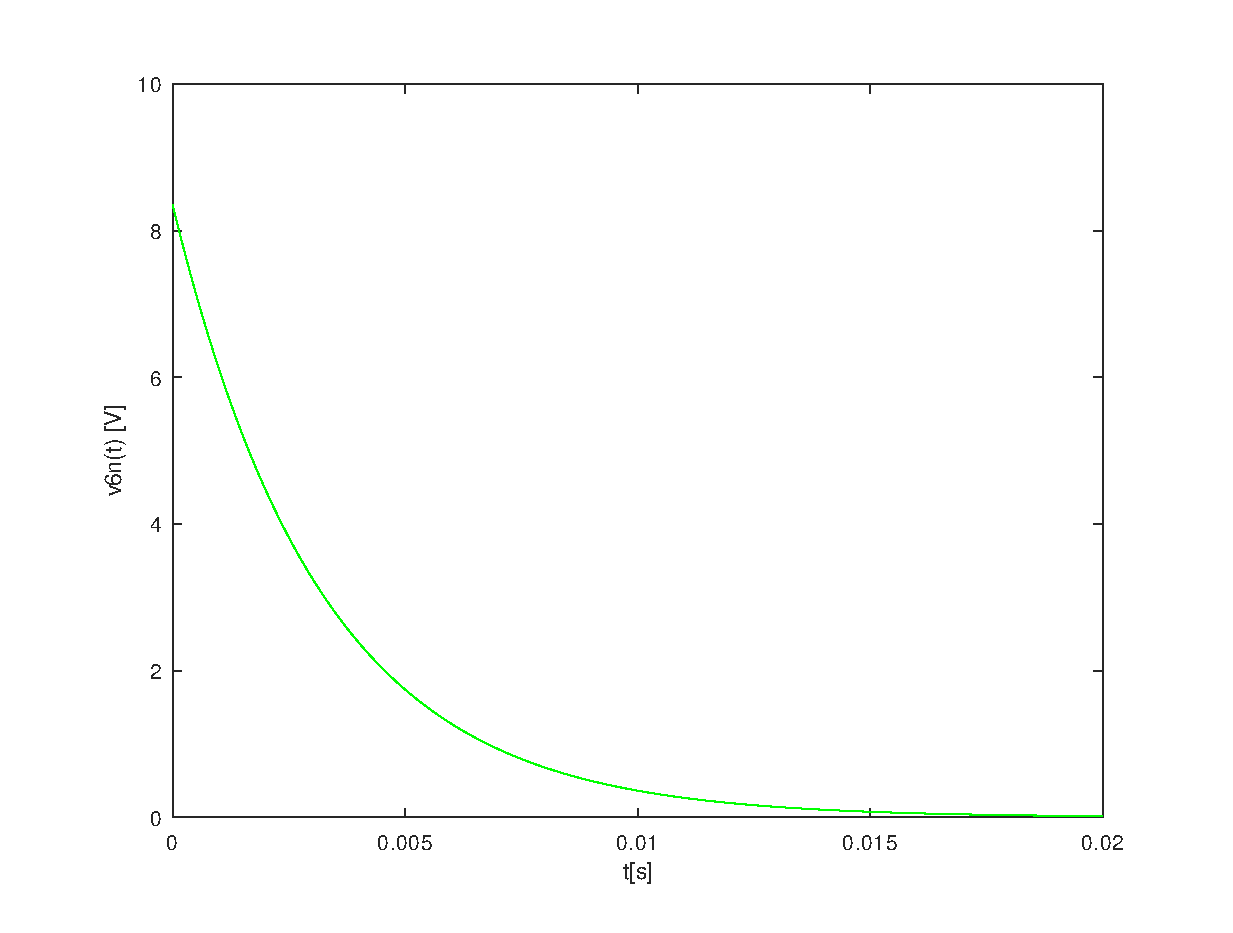
\includegraphics[width=0.9\linewidth, height=6cm]{natural.eps} 
\caption{The natural solution, $V6_n(t)$, during time interval [0, 20] ms, obtained using GNU Octave.}
\label{fig:theo_third}
\end{subfigure}
\begin{subfigure}{0.5\textwidth}
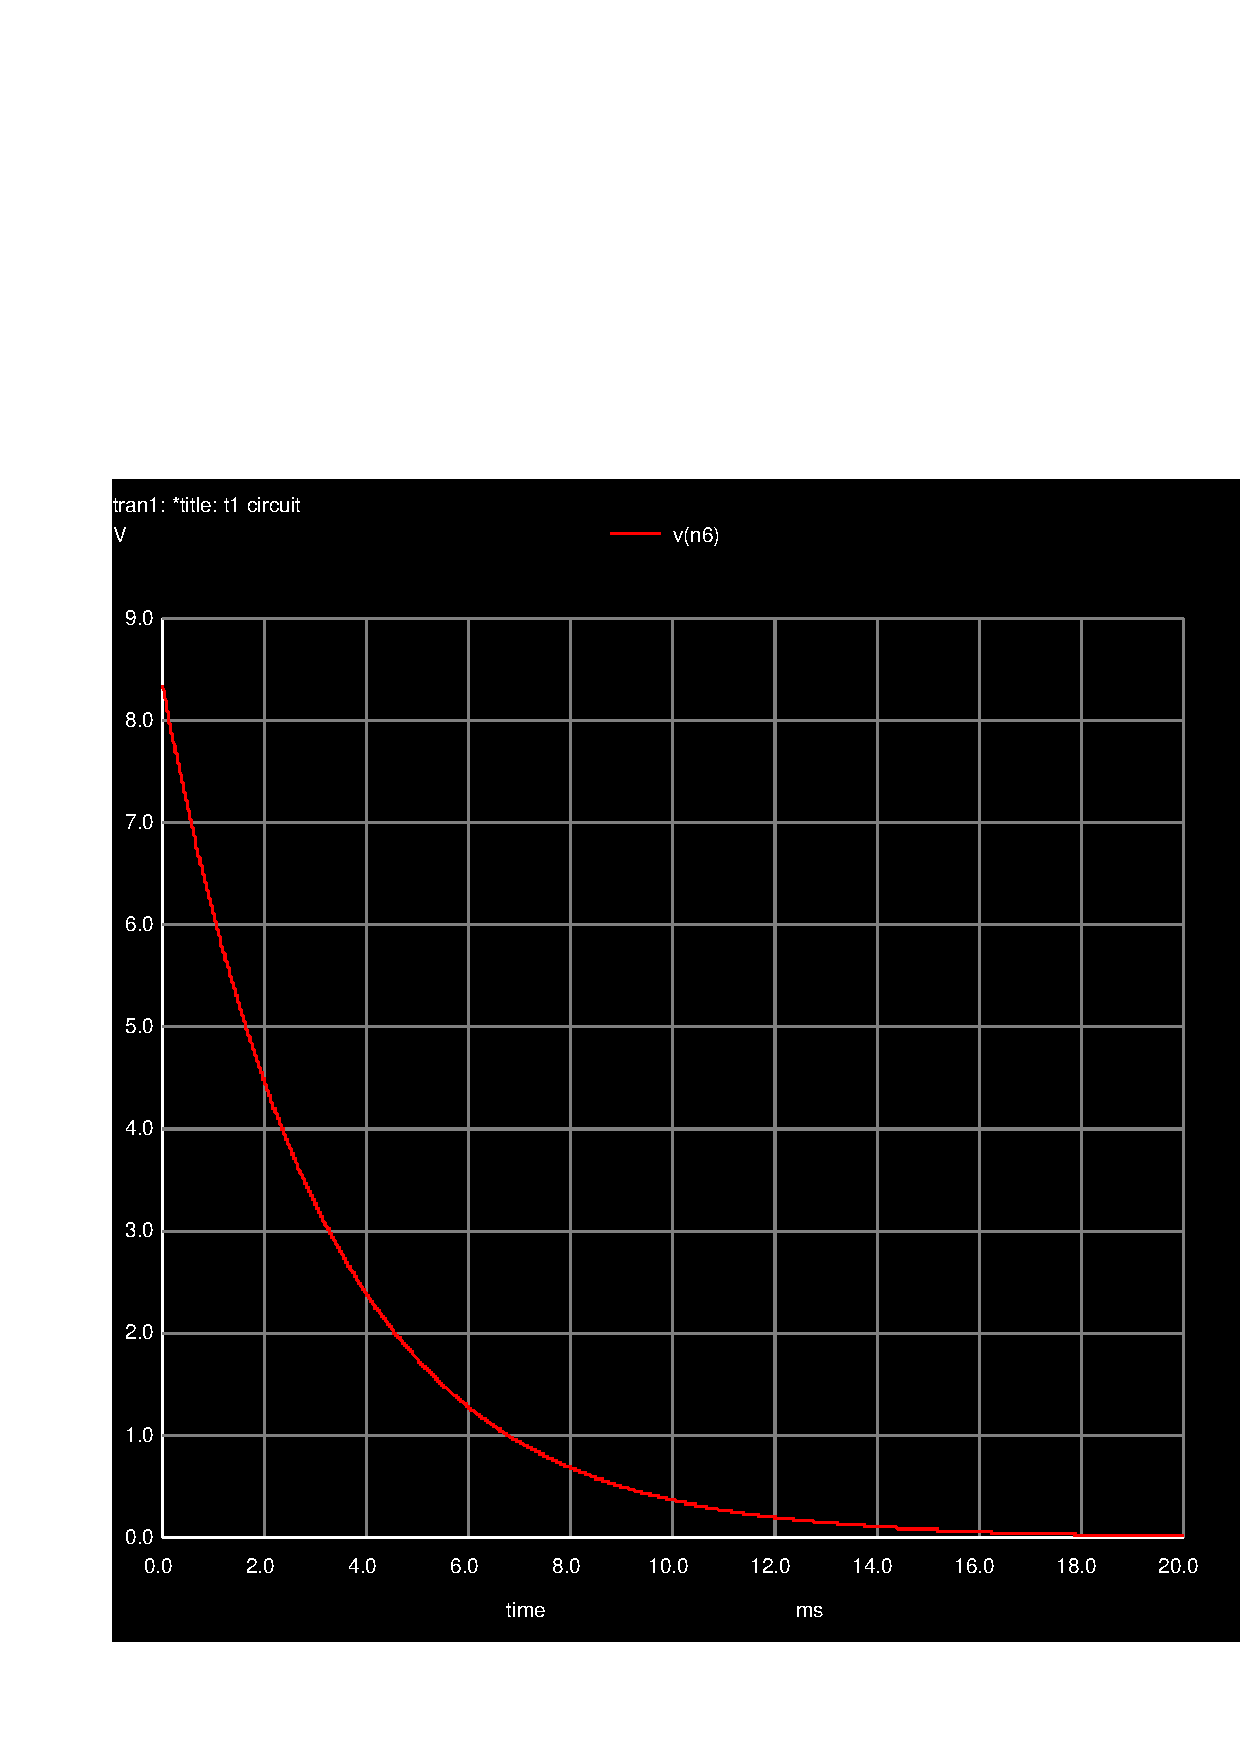
\includegraphics[width=0.9\linewidth, height=6cm]{trans1.pdf}
\caption{The natural solution, $V6_n(t)$, during time interval [0, 20] ms, obtained using Ngspice.}
\label{fig:natural}
\end{subfigure}

\caption{Comparation of theoretical and simulation analysis for the natural response.}
\label{fig:compar_1}
\end{figure}

\paragraph{}
When the simulation graphic given by Ngspice in Section~\ref{sec:simulation} is compared to the theoretical one obtained in Section~\ref{sec:analysis}, it is possible to highlight the fact that these are, in reality, extremely close to each other. As it can be seen, both of the graphics describe a very similar descendent curve. The natural response of the electric circuit provocates a descent in the node voltage value, which tends to stabilize by the end of the time interval.

\subsection{Topic Theo V - Sim IV}
\label{subsec:fourth_topic_error}

\begin{figure}[H]

\begin{subfigure}{0.5\textwidth}
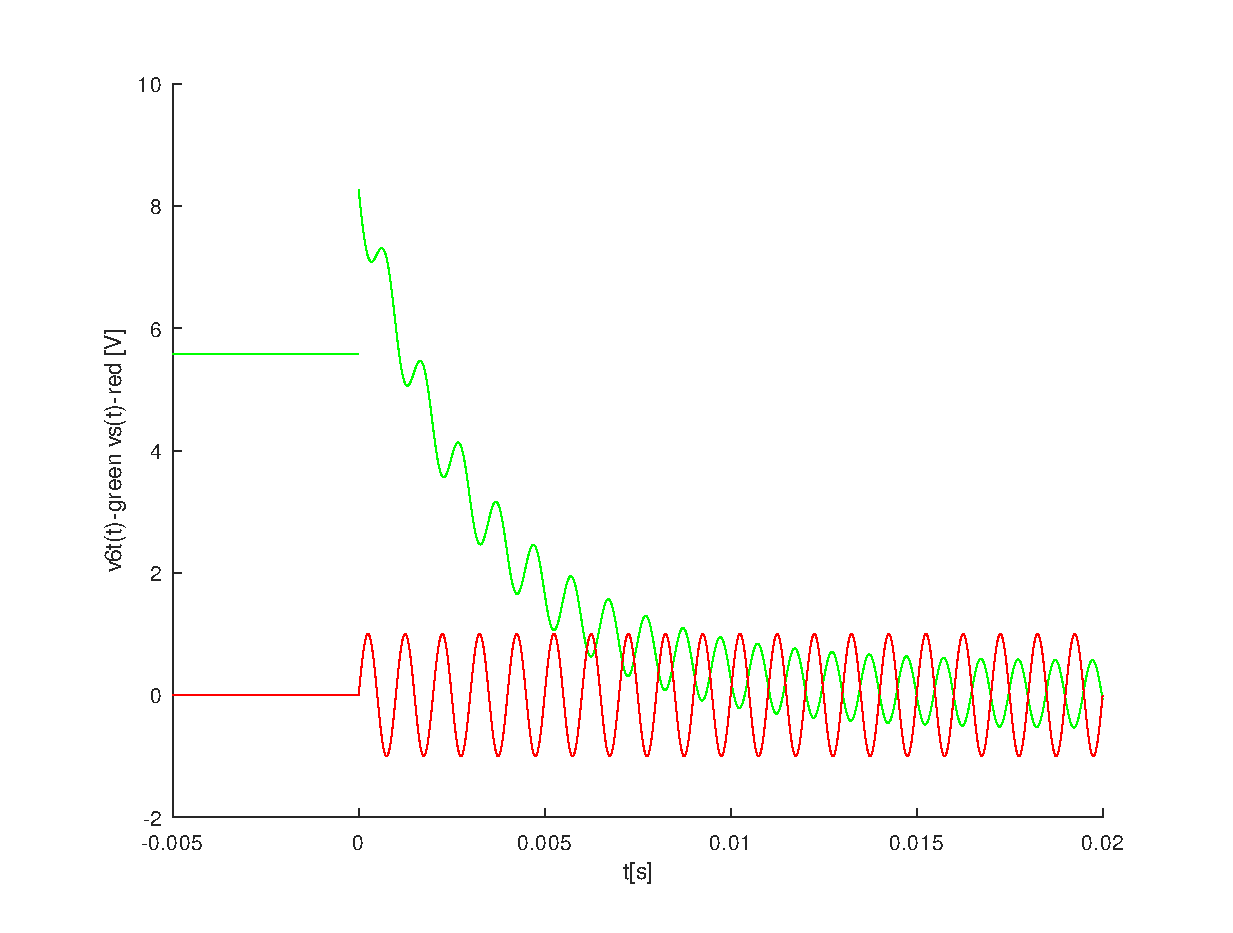
\includegraphics[width=0.9\linewidth, height=6cm]{total.eps} 
\caption{The final total solution, $V6(t)$,  and $v_s(t)$ during time interval [-5, 20] ms, obtained using GNU Octave.}
\label{fig:theo_fifth}
\end{subfigure}
\begin{subfigure}{0.5\textwidth}
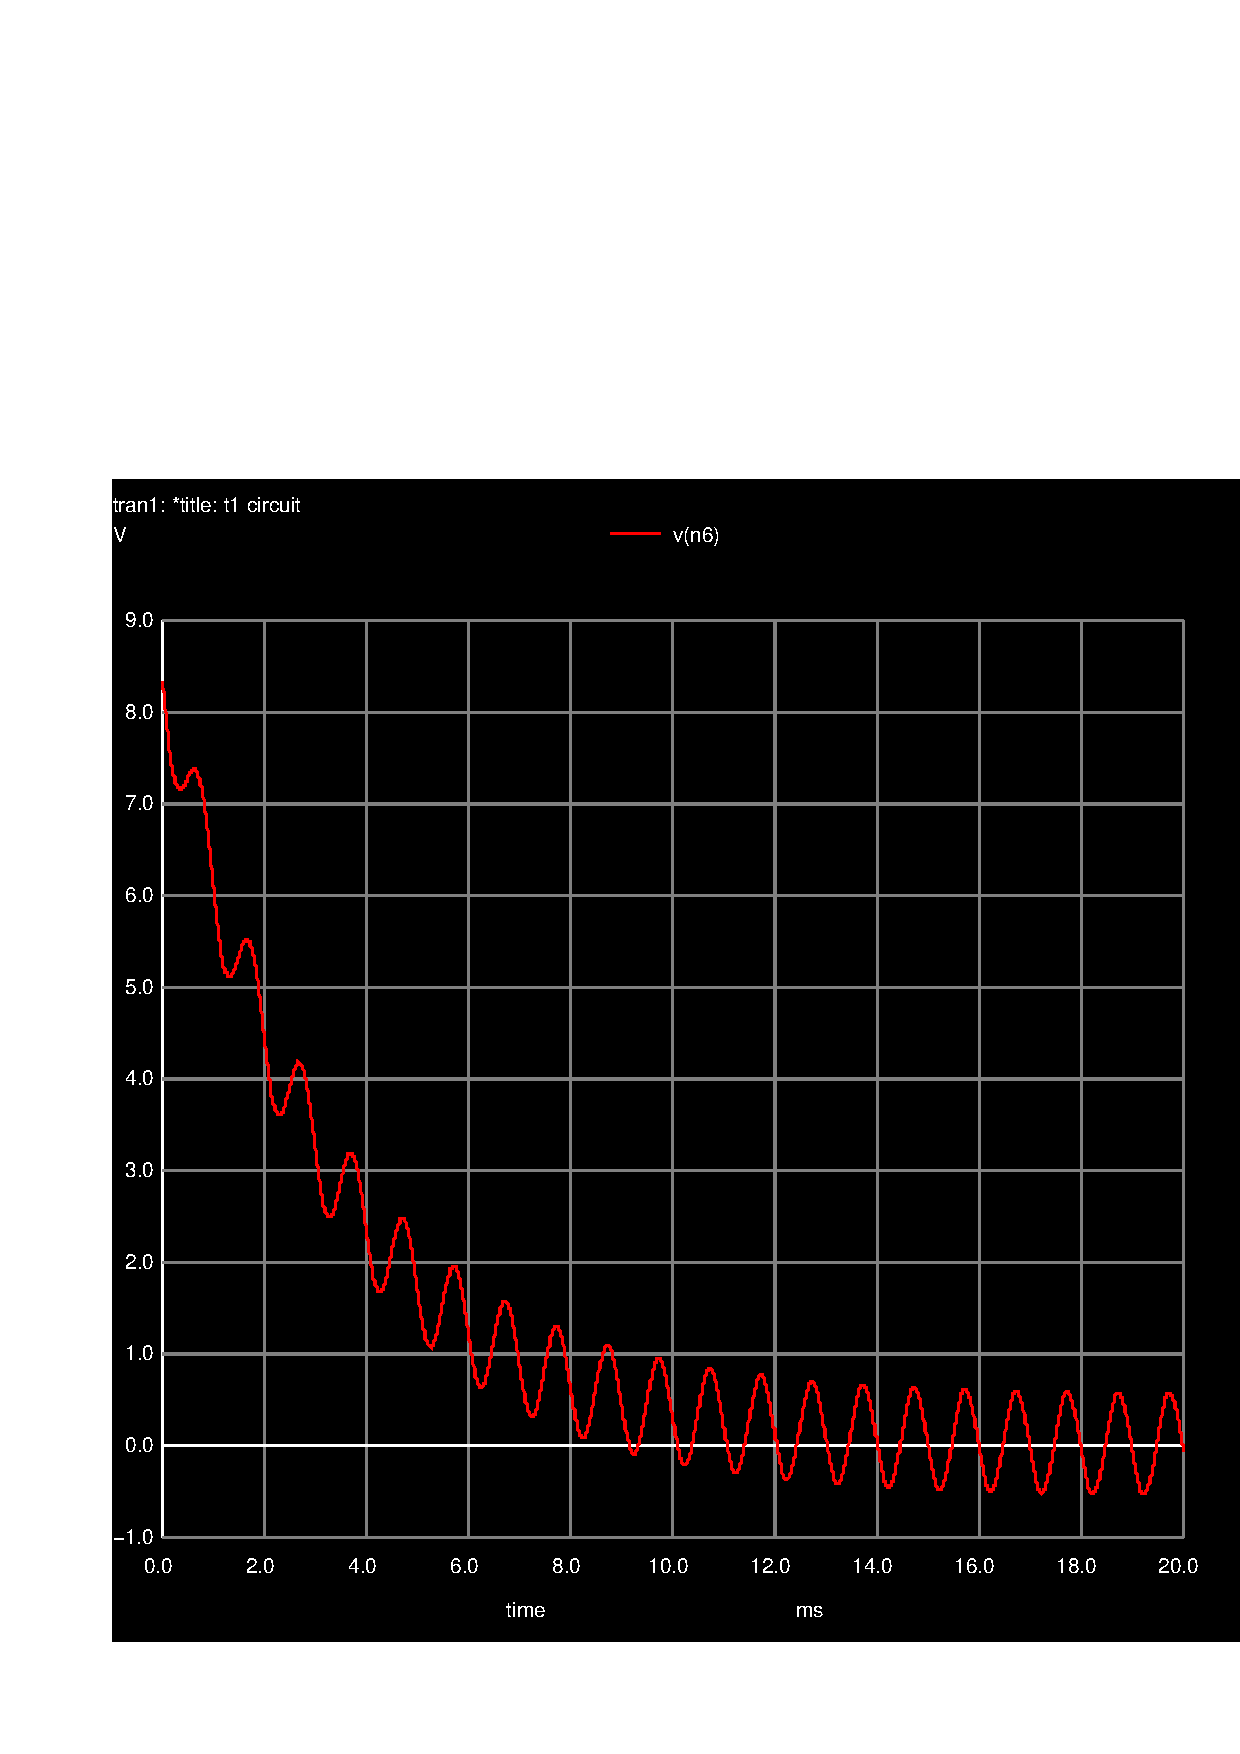
\includegraphics[width=0.9\linewidth, height=6cm]{trans2.pdf}
\caption{The final total solution, $V6(t)$, during time interval [-5, 20] ms, obtained using Ngspice.}
\label{fig:total}
\end{subfigure}

\caption{Comparation of theoretical and simulation analysis for the total response.}
\label{fig:compar_2}
\end{figure}

\paragraph{}
When the simulation graphic given by Ngspice in Section~\ref{sec:simulation} is compared to the theoretical one obtained in Section~\ref{sec:analysis}, it is possible to highlight the fact that these are, in reality, extremely close to each other. As it can be seen, both of the graphics describe a very similar descendent curve with a certain oscilation. This variation of the node voltage along the curve seems to be constant in the two graphic representations. The total response of the electric circuit provocates a descent in the node voltage value, which tends to stabilize by the end of the time interval.


\subsection{Topic Theo VI - Sim V}
\label{subsec:fifth_topic_error}

\begin{figure}[H]

\begin{subfigure}{0.5\textwidth}
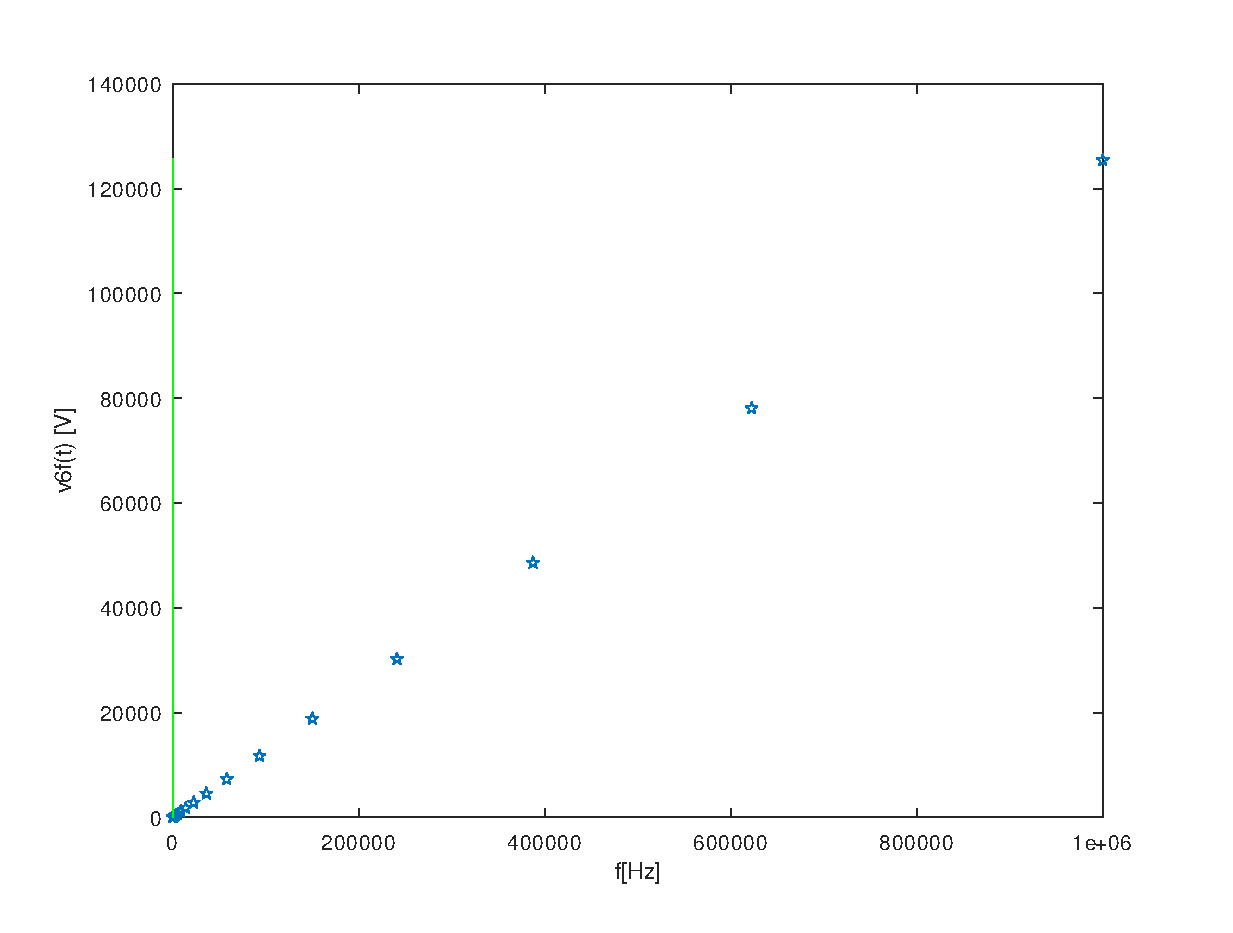
\includegraphics[width=0.9\linewidth, height=6cm]{magnitude.eps} 
\caption{Magnitude of $v_s(f)$,  $v_c(f)$  and $v_6(f)$ during frequency interval [0.1 , 1] MHz, obtained using GNU Octave}
\label{fig:theo_third}
\end{subfigure}
\begin{subfigure}{0.5\textwidth}
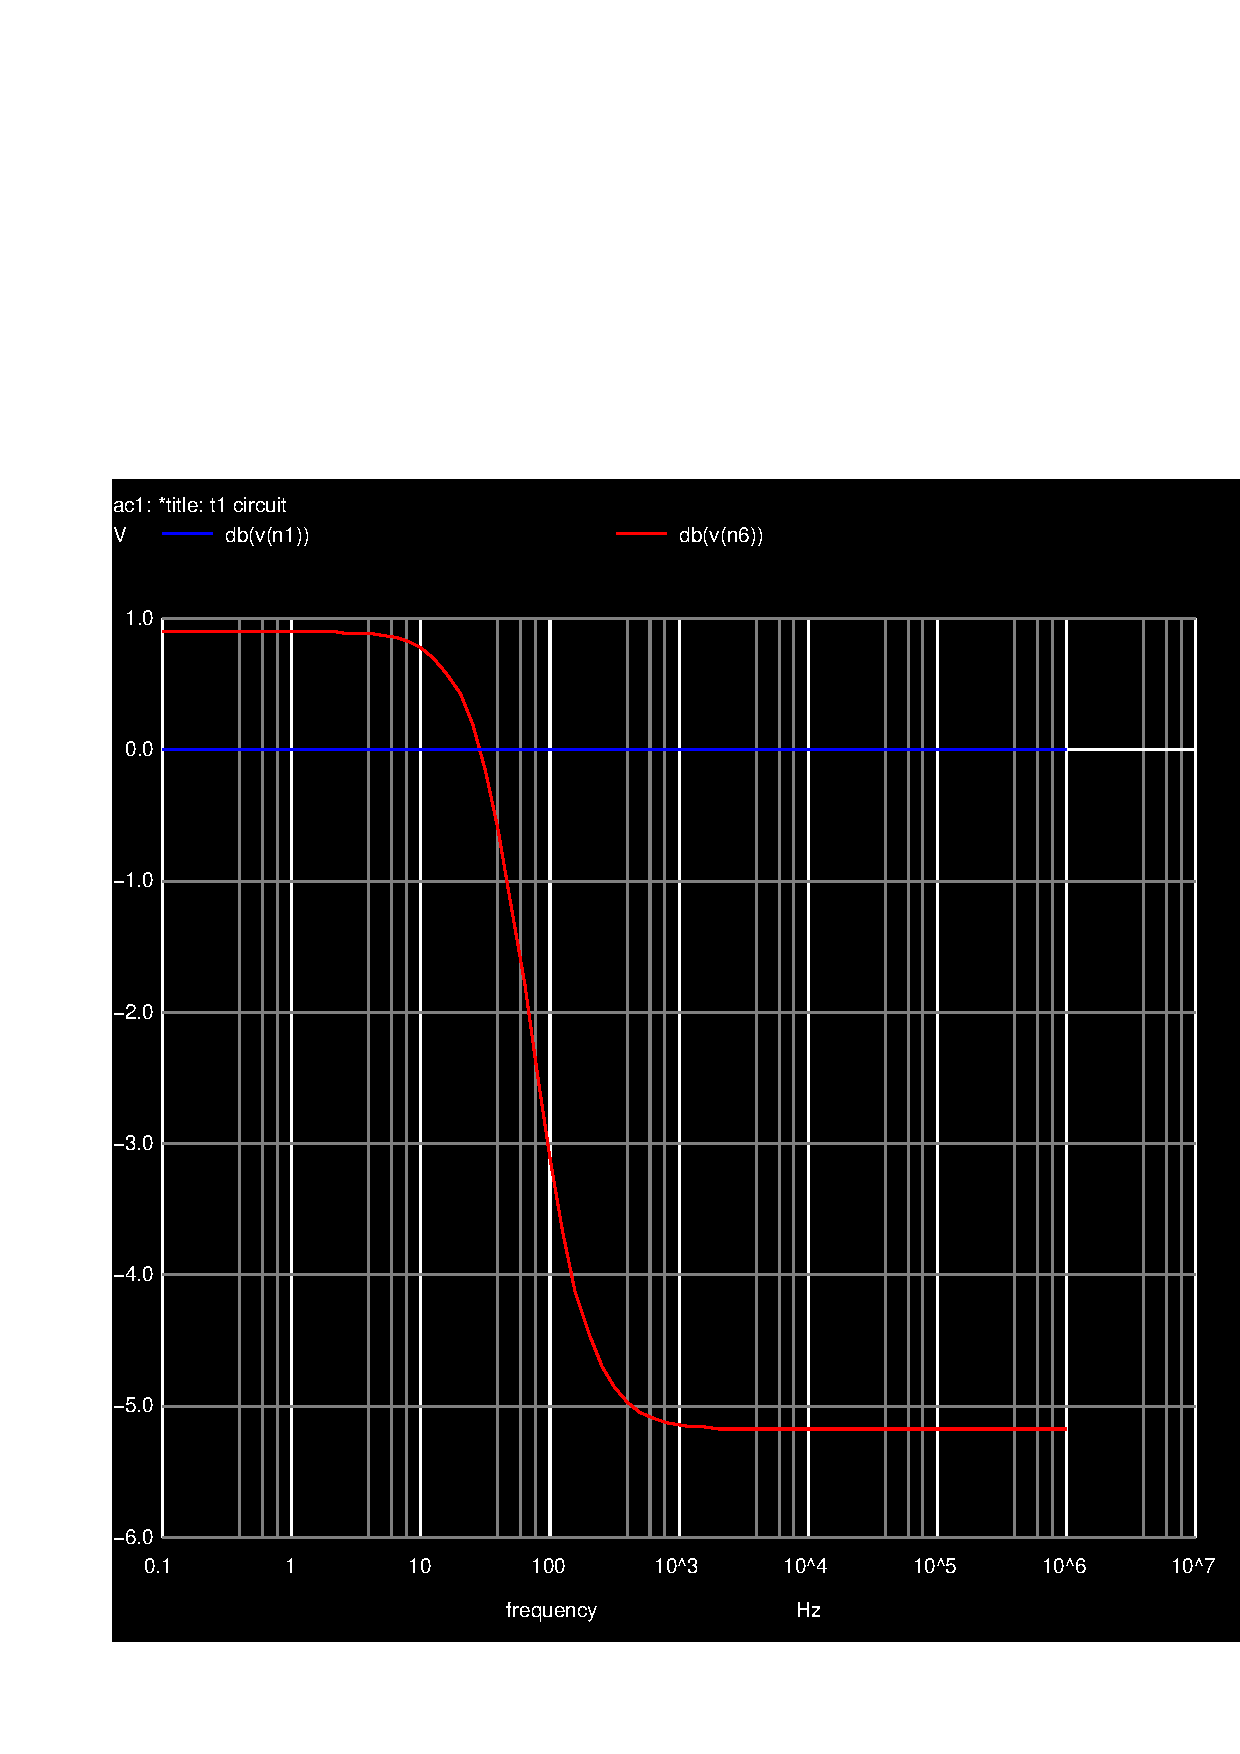
\includegraphics[width=0.9\linewidth, height=6cm]{acm.pdf}
\caption{Magnitude of $v_s(f)$ and $v_6(f)$ during frequency interval [0.1 , 1] MHz, obtained using Ngspice.}
\label{fig:total}
\end{subfigure}

\caption{Comparation of theoretical and simulation analysis for the nodal voltage magnitude.}
\label{fig:compar_3}
\end{figure}

\paragraph{}
When the simulation graphic given by Ngspice in Section~\ref{sec:simulation} is compared to the theoretical one obtained in Section~\ref{sec:analysis}, it is possible to highlight the fact that these are, in reality, extremely close to each other. As it can be seen, the magnitude of $v_s$ is null and it remains constant till the end of the time interval. On the other hand, the magnitude of node voltage $V_6$ is represented by a curve that shows variation through time. This magnitude is described by a descent of the node voltage values, which start with a constant value around 1 db and tends to stabilize near -5 db in the final section of the interval. This values can be evaluated both in theoretical and simulation graphics, which represent the exact same curve with an inflexion point in the middle value of the time interval.


\begin{figure}[H]

\begin{subfigure}{0.5\textwidth}
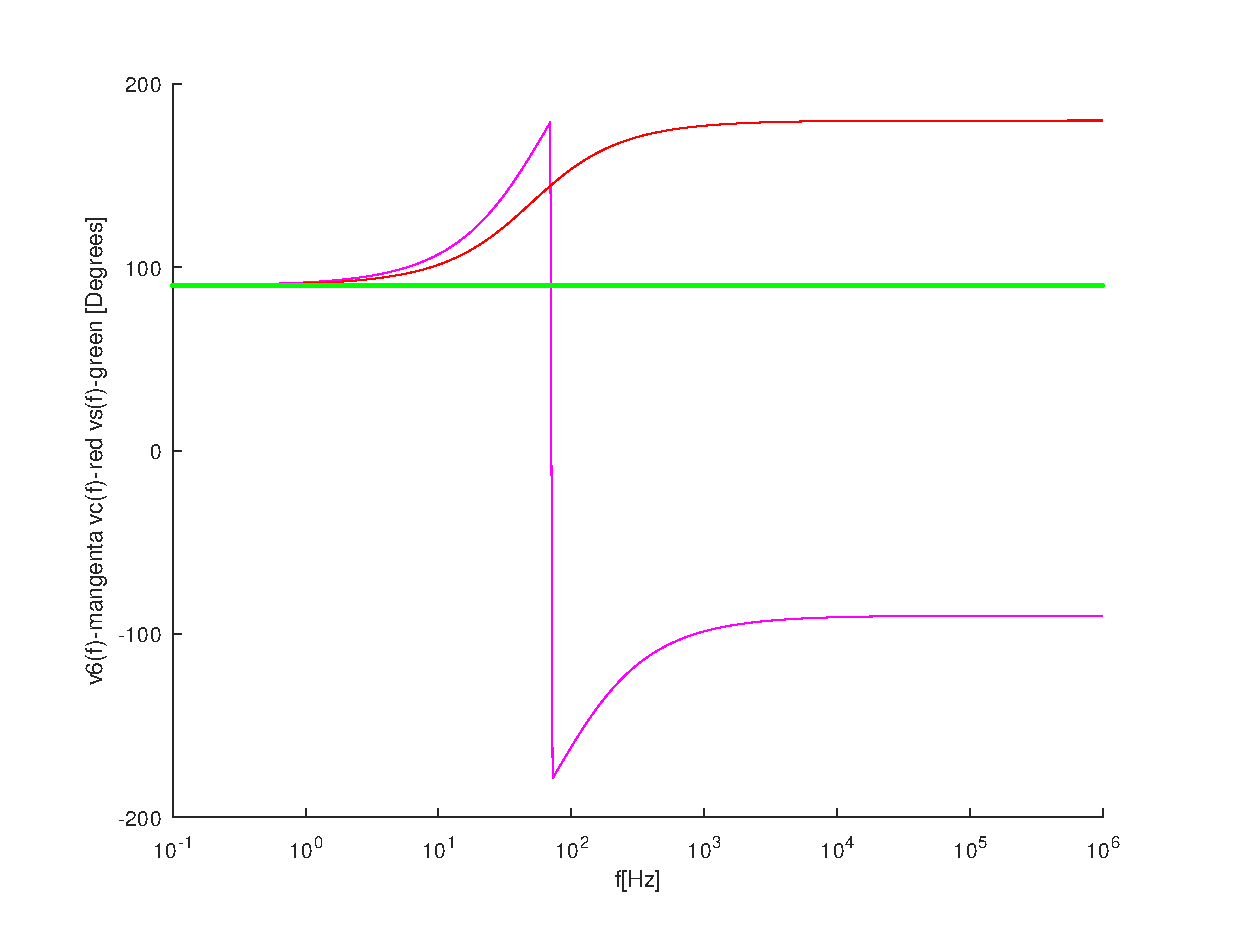
\includegraphics[width=0.9\linewidth, height=6cm]{phase.eps} 
\caption{Phase $v_s(f)$,  $v_c(f)$  and $v_6(f)$ during frequency interval [0.1 , 1] MHz, obtained using GNU Octave.}
\label{fig:theo_third}
\end{subfigure}
\begin{subfigure}{0.5\textwidth}
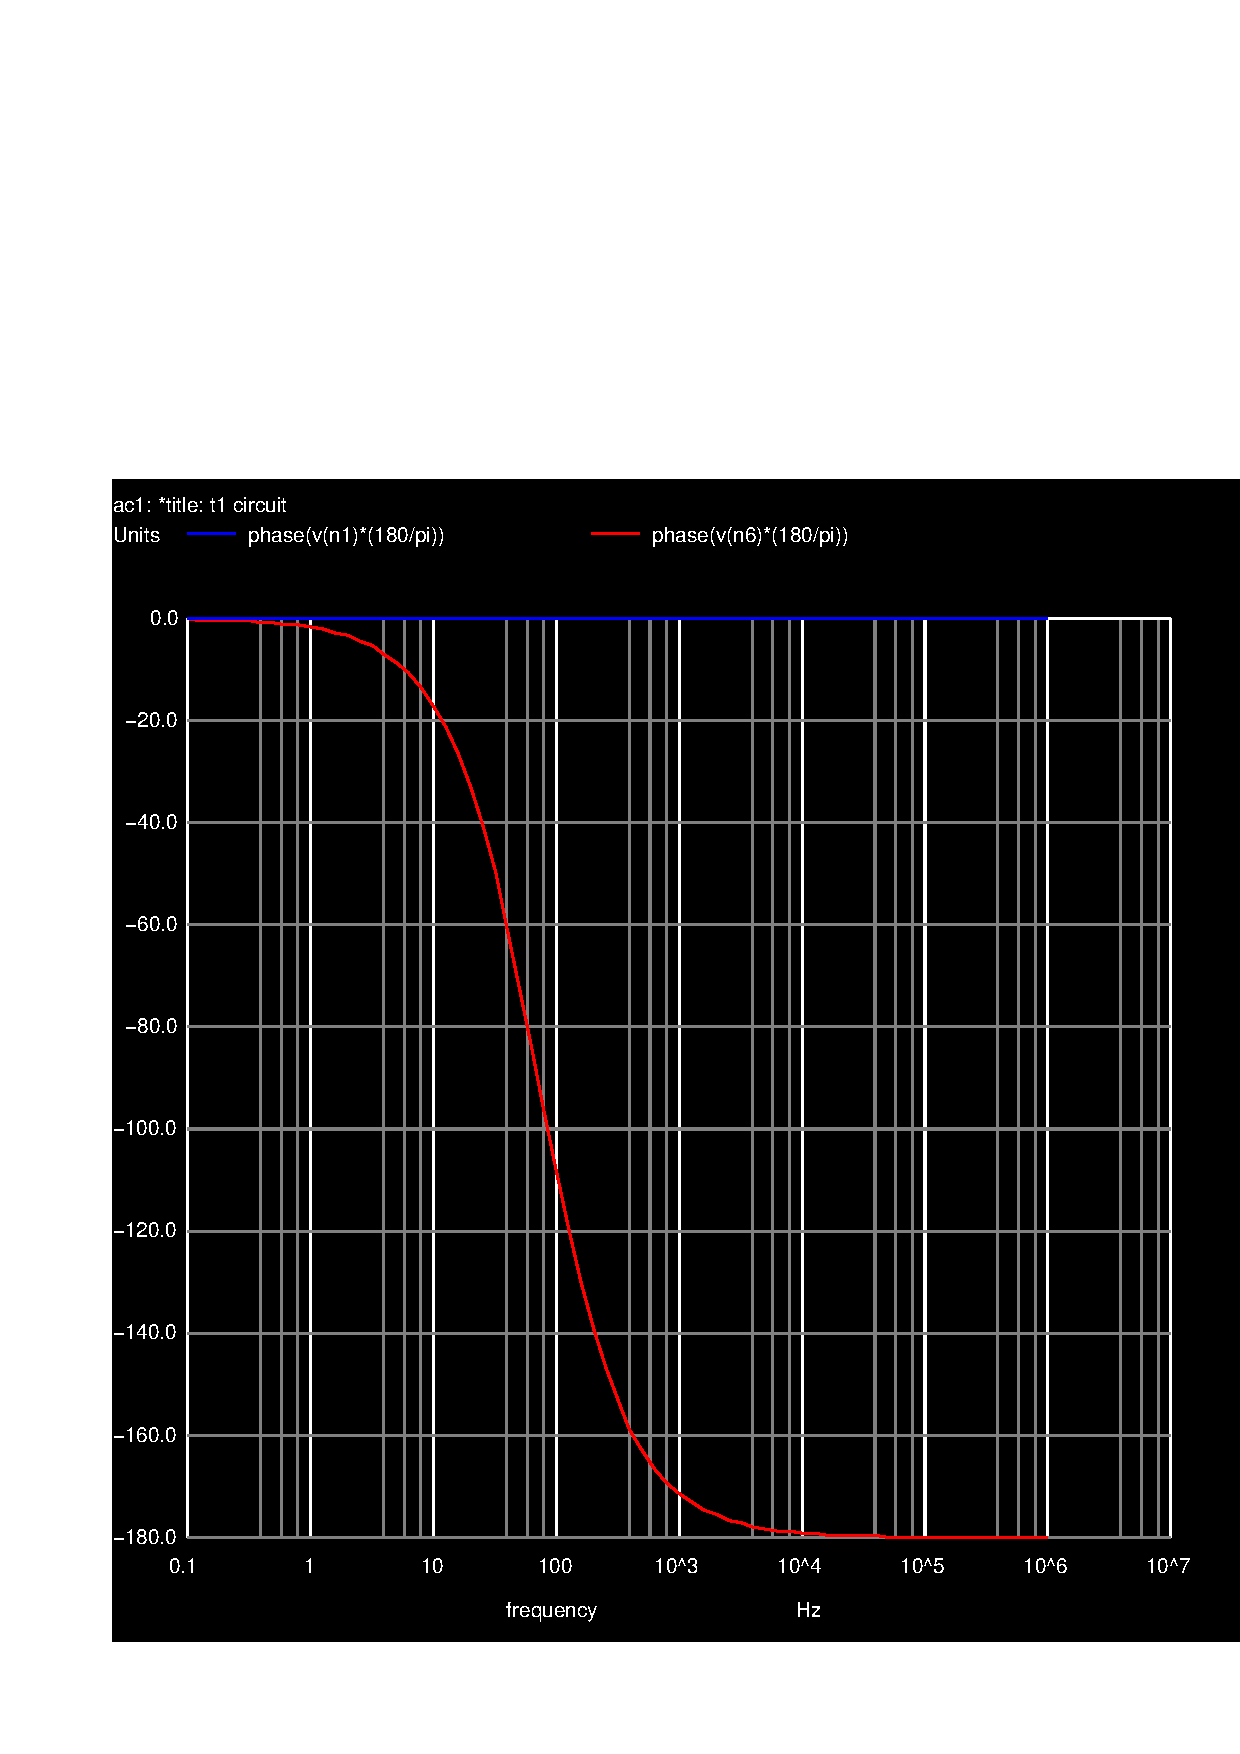
\includegraphics[width=0.9\linewidth, height=6cm]{acp.pdf}
\caption{Phase of $v_s(f)$ and $v_6(f)$ during frequency interval [0.1 , 1] MHz. obtained using Ngspice.}
\label{fig:total}
\end{subfigure}

\caption{Comparation of theoretical and simulation analysis for the nodal voltage phase.}
\label{fig:compar_4}
\end{figure}

\paragraph{}
When the simulation graphic given by Ngspice in Section~\ref{sec:simulation} is compared to the theoretical one obtained in Section~\ref{sec:analysis}, it is possible to highlight the fact that these are, in reality, extremely close to each other. As previously stated for the magnitude, also the phase of $v_s$ is null and remains constant till the end of the time interval. On the other hand, the phase of node voltage $V_6$ is also null in the beggining of the time interval. However, as we can see, the phase of this node voltage is represented by a curve that shows a descent variation through time. This phase can be described by this curve with an inflexion point in the middle value of the time interval that tends to stabilize near -100 degrees. Once more, all the values can be evaluated both in theoretical and simulation graphics, that proved to be really close to each other.















